\documentclass[a4paper, 10pt]{article}
\usepackage{header}

% \usepackage{pgfplots}


\title{\LARGE{Microeconomics-2 (advanced course)}\\
FES HSE}
\author{Viner Daniil  \href{https://t.me/danya_vin}{@danya\_vin}}
\date{Last update \today}

\begin{document}
\maketitle
\tableofcontents
\newpage
\setlength{\parindent}{15pt}
\setlength{\parskip}{2mm}
\setlist[itemize]{left=1cm}
\setlist[enumerate]{left=1cm}
\section{Classic monopoly}
\subsection{Definition}
A firm is \textbf{a monopoly} if no other firms produces the same good or a close substitute.

\comment We differentiate among the products referring to the cross-price elasticity: if its value is small, then the potential substitutes are not close enough to be a substitute.

A monopolist has market power in the sense that the amount of output that it is able to sell responds continuously on the price it charges.

Obviously, that the monopolist suggests consumers a good at a price of $p$. 

\subsection{Examples of a monopoly}
The main reason why a monopoly exists is the fact that other firms find it impossible or unprofitable to enter the market (or to continue the competition with more bigger firms).

The greatest examples of a monopoly are:
\begin{itemize}
    \item Natural monopolies, when a single company can produce and offer to sell a product or service at a lower cost than its competitors can
    \item Legal protection of a patent holder, when the government prohibits using some technologies, ideas and producing methods except by those who created them
\end{itemize}


\subsection{Model of a monopoly}
Let’s suppose there are many consumers of a good and they are price-takers. We'll assume that a good which we're considering is normal, which means that the function of demand — $D(p)$ is decreasing.

$y=D(p)$ — the output if the monopoly, $c(y)$ — costs function of the firm-monopolist.

So, the monopolist chooses the price $p^m$ which is the solution of the maximization problem:
\begin{equation}\label{eq:1.3.1}
    \Pi(p)=pD(s)-c(D(p))\longrightarrow\max_{p\geqslant0}
\end{equation}

Logically, $y^m=D(p^m)$ is the output of the monopolist.

Sometimes it's easier to use an inverse function $p=p(y)=D^{-1}(y)$.

Then, output $y^m$ is the solution of this problem:
\begin{equation}\label{eq:1.3.2}
    \Pi(y)=p(y)y-c(y)\longrightarrow\max_{y\geqslant0}
\end{equation}

\subsection{First-order condition}
\begin{equation}
    \begin{cases}
        \Pi'(y^m)\leqslant 0\\
        y^m\cdot\Pi(y^m)=0
    \end{cases}
\end{equation}
\indent Condition that $y^m>0$ is guaranteed by:
\begin{equation}
    p(0)>c'(0)
\end{equation}

\textbf{Proof.} If $y^m=0$, next condition must be done:
\begin{equation*}
    \Pi'(0)=p(0)-c'(0)\leqslant 0
\end{equation*}
which contradicts $p(0)>c'(0)$\qed

\begin{equation}
    \begin{aligned}
        \Pi(y)&=p(y)y-c(y)\\
        \Pi'(y)&=\left(p(y)y-c(y)\right)^{\prime}=0\\
        &=p(y)\cdot p'(y)y=c'(y),\quad \text{at }y=y^m>0
    \end{aligned}
\end{equation}

Then, $p^m=p(y^m)$

Let's $TC=D(p)p$, $TC=c(D(p))$, then as we maximize $\Pi$
\begin{equation*}
    \begin{aligned}
        \Pi'&=0\\
        TR'-TC'&=0\\
        MR-MC&=0
    \end{aligned}
\end{equation*}

$$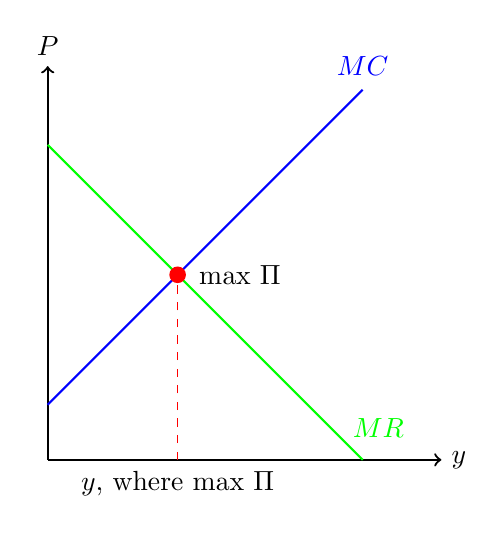
\begin{tikzpicture}[scale=2]

    \draw[thick,->] (0,0) -- (2.5,0) node[right] {$y$}; 
    \draw[thick,->] (0,0) -- (0,2.5) node[above] {$P$}; 

    \draw[thick, green] (0,2) -- (2,0);
    \draw[thick, blue] (0,0.35) -- (2,2.35);
    
    \fill[red] (0.825,1.175) circle (1.5pt);
    \node[anchor=west, black] at (0.9,1.175) {max $\Pi$};

    \draw[dashed, red] (0.825,0) -- (0.825,1.175);

    \node[black] at (0.825,-0.15) {$y$, where max $\Pi$};
    \node[blue] at (2,2.5) {$MC$};
    \node[green] at (2.1,0.2) {$MR$};

\end{tikzpicture}$$
\subsection{Second-order condition}
Let $TR(y)=p(y)y$ and $MR(y)=TR'(y)$, then
\begin{equation}
    \left(MR(y^m)\right)'<\left(MC(y^m)\right)'
\end{equation}
\subsection{Illustration of the monopolist problem}
$$
\begin{tikzpicture}[scale=2]

    \draw[thick,->] (0,0) -- (4,0) node[right] {$y$}; 
    \draw[thick,->] (0,0) -- (0,4) node[above] {$P$};

    \draw[thick, blue] (0,3.5) -- (1.9,0); %MC
    \draw[thick, green] (0.5,1) .. controls (2,1) and (2,2.2) .. (2.05,2.2); %MR 
    \draw[thick, red] (0,3.5) -- (3.8,0);

    \fill[teal] (1.28,2.33) circle (1.5pt);


    \draw[dashed, teal] (1.28,0) -- (1.28,2.33);
    \draw[dashed, teal] (0,2.33) -- (1.28,2.33);
    \node[anchor=east, teal] at (0,2.33) {$p^m$};
    \node[anchor=north east, teal] at (1.38,0) {$y^m$};
    \node[anchor=north west, blue] at (1.9,0.3) {$MR$};
    \node[anchor=north west, red] at (3.6,0.5) {$p(y)=D^{-1}(y)$};
    \node[green] at (2.2,2.1) {$MC$};
    
\end{tikzpicture}
$$

Here $p^m$ and $y^m$ are the price and output at which customers will buy the volume of good at which $MR=MC$.

\subsection{Inverse elasticity pricing rule}
\definition 
\begin{equation}\label{eq:1.7.1}
    \frac{p^m-MC(y^m)}{p^m}=\frac{1}{|\varepsilon_d|},\quad \text{for }|\varepsilon_d|>1
\end{equation}

The right part of the formula (\ref{eq:1.7.1}) is called \textbf{Lerner's Index}. It shows the degree of the monopoly power. At the same time it shows how the mark-up price depends on the elasticity of demand. 

\comment If the elasticity of demand is infinite, then the firm is a price taker and has no market power.

\comment The greater the elasticity, the smaller the markup the manufacturer can make because in that case customers will refuse to consume.

Let's find the formula (\ref{eq:1.7.1}) by mathematical transformation. We know that:
\begin{itemize}
    \item $p'(y^m)y^m+p(y^m)=c'(y^m)$
    \item $p(y^m)=c'(y^m)$
    \item $\varepsilon_d=\displaystyle\frac{\text{d}y}{\text{d} p}\cdot\frac{p}{y}<0$
\end{itemize}
So, transform by using that equations we get
$$\begin{aligned}
    p(y^m)\left[1+\displaystyle\frac{p'(y^m)y^m}{p(y^m)}\right]&=c'(y^m)\\
    p^m\left[1-\displaystyle\frac{1}{|\varepsilon_d|}\right]&=c'(y^m)\\
    p^m-\displaystyle\frac{p^m}{|\varepsilon_d|}&=c'(y^m)\\
    \displaystyle\frac{p^m-c'(y^m)}{p^m}&=\frac{1}{|\varepsilon_d|}\\
    \frac{p^m-MC(y^m)}{p^m}&=\frac{1}{|\varepsilon_d|}
\end{aligned}$$

\subsection{Monopoly's output in comparison with the perfectly competitive industry}
Consider a monopoly with the $c(y) \in C^1$ costs function and a perfectly competitive industry with the same costs $c(y)$.Let $p(y) \in C^1$ be an inverse demand function. Then given $p' > 0,\ c' > 0,\ c'' > 0$ and $p(0) > c'(0)$

\noindent
\begin{minipage}{0.5\textwidth}
\proposition The monopoly output $y^m$ will be less than the output $\overline{y}$ of the perfectly competitive industry
\begin{equation}\label{eq:1.8.1}
    y^m<\overline{y}
\end{equation}

\proof It's simple. On the one hand, $y^m$ maximizes $\Pi$ of the monopoly, then
$$p(y^m)y^m-c(y^m)\geqslant p(\overline{y})\overline{y}-c(\overline{y})$$

On the other hand, $\overline{y}$ provides maximum profit to the price-taking firm at a constant price $p(\overline{y})$, then
$$p(\ov{y})\ov{y}-c(\ov{y})\geqslant p(\ov{y})y^m-c(y^m)$$

Adding these equations we get $p(y^m)y^m\geqslant p(\ov{y})y^m\Longrightarrow\boxed{y^m<\ov{y}}$\footnote{Remember, that $p(y)$ is an inverse function of demand and $y^m\ne \ov{y}$ because of $p(\ov{y})-c'(\ov{y})\leqslant0$}
\end{minipage}
\begin{minipage}{0.5\textwidth}
$$
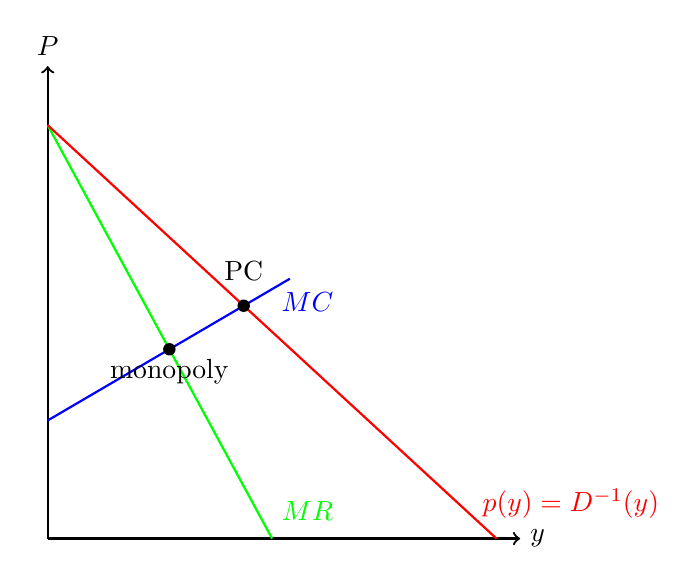
\begin{tikzpicture}[scale=1.5]

    \draw[thick,->] (0,0) -- (4,0) node[right] {$y$}; 
    \draw[thick,->] (0,0) -- (0,4) node[above] {$P$};

    \draw[thick, green] (0,3.5) -- (1.9,0); 
    \draw[thick, blue] (0,1) -- (2.05,2.2); 
    \draw[thick, red] (0,3.5) -- (3.8,0); %p(y)

    \fill[teal, black] (1.02988, 1.60286) circle (1.5pt);
    \fill[teal, black] (1.65957, 1.97145) circle (1.5pt);

    \node[anchor=north west, green] at (1.9,0.4) {$MR$};
    \node[anchor=north west, red] at (3.6,0.5) {$p(y)=D^{-1}(y)$};
    \node[blue] at (2.2,2) {$MC$};
    \node[anchor=south, black] at (1.65957, 2.1) {\text{PC}};
    \node[anchor=north, black] at (1.02988, 1.60286) {\text{monopoly}};
    
\end{tikzpicture}
$$
\end{minipage}
\subsection{Comparative Statics}
Let $p(y)\in C^2,\ p' <0,\ MC =c,\ p(0)>c,\ (MR)' <0$. Then
\begin{equation*}
    \frac{dy^m(c)}{dc}<0\quad \text{and}\quad\frac{dp^m(c)}{dc}>0
\end{equation*}

\section{Quasilinear Economy}
Consider an economy where there are $m$ consumers and $n$ firms. All of consumers have quasilinear preferences, for $i$-th consumer his utility is $U_i(x_i,z_i)=v_i(x_i)+z_i$, where $x_i$ is the only good to be consumed and $z_i$ is the money owned by this consumer.

Properties of $v_i(x_i)$ functions:
\begin{itemize}
    \item $v_i'(x_i)>0$
    \item $v_i''(x_i)<0$
    \item $v_i(0)=0$
\end{itemize}

\subsection{Main theorem of the quasilinear economy}
Let $\bar{x}=\left(x_1, x_2, \ldots, x_m\right), \bar{y}=\left(y_1, y_2, \ldots, y_n\right), \bar{r}=\left(r_1, r_2, \ldots, r_n\right)$ and $\bar{z}=\left(z_1, z_2, \ldots, z_m\right)$

Allocation $(\widehat{\bar{x}}, \widehat{\bar{y}}, \widehat{\hat{r}}, \widehat{\bar{z}})$ is Pareto-optimal if and only if it is a solution of the problem
\begin{equation}\label{eq:2.1.1}
\left\{\begin{array}{l}
\sum_i \nu_i\left(x_i\right)-\sum_j c_j\left(y_j\right) \longrightarrow \max \\
\sum_i\left(x_i\right) \leq \sum_i y_j \\
x_i \geq 0,\ y_j \geq 0 \\
\text {for all } i \in I \text { and } j \in J
\end{array}\right.
\end{equation}


Moreover $\widehat{r_j}=c_j\left(\widehat{y_j}\right)$ and $\sum_i \widehat{z_i}=\sum_i w_i-\sum_j \widehat{r_j}$.

\subsection{Welfare analysis under monopoly}
The first line in (\ref{eq:2.1.1}) is the main goal of consumers, i.e. to maximize the welfare. That function is called a \textbf{welfare indicator}. Then we have $2$ sets of indices, $I = \{1,2,\ldots,m\}$ and
$J = \{1,2,\ldots,n\}$.

At \textit{Pareto-optimal allocation} it takes the maximum value $W_{max}$. If an allocation \textit{is not} Pareto-optimal, then $W < W_{max}$ and this difference $W_{max} - W$ is called \textbf{deadweight loss} $(DWL)$.

We give the following definitions for Consumers’ ($CS$) and producers’ ($PS$) surplus:
\begin{equation}
    \begin{aligned}
        CS&=&\sum_{i\in I}\nu_i(x_i)-p\sum_{i\in I}x_i\\
        PS&=&p\sum_{j\in J}y_j-\sum_{j\in J}c_j(y_j)
    \end{aligned}
\end{equation}

Welfare indicator at $(x, y)$ allocation equals $W (x, y) = CS + PS$. Moreover, we can identify $$W=\sum_{i=1}^m v_i(x_i)-c(y)$$

Let $y=\sum_{i\in I}x_i=x$ — output of a monopoly

\begin{enumerate}
    \item $W(y)=v(y)-c(y)\longrightarrow\max\limits_{y>0}\Longrightarrow v'(y)=c'(y)$
    \item First-order condition:
    \begin{equation*}
        \begin{aligned}
            \left(p(y)y\right)'-c'(y)&=0\\
            p'(y)y+p(y)-c'(y)&=0
        \end{aligned}
    \end{equation*}
    \item If we differentiate the formula $W(y)=v(y)-c(y)$:
    \begin{equation*}
        \begin{aligned}
            W'(y^m)&=v'(y^m)-c'(y^m)>0\\
            &=p(y^m)-c'(y^m)\\
            &=-p'(y^m)y^m>0
        \end{aligned}
    \end{equation*}
\end{enumerate}

$$
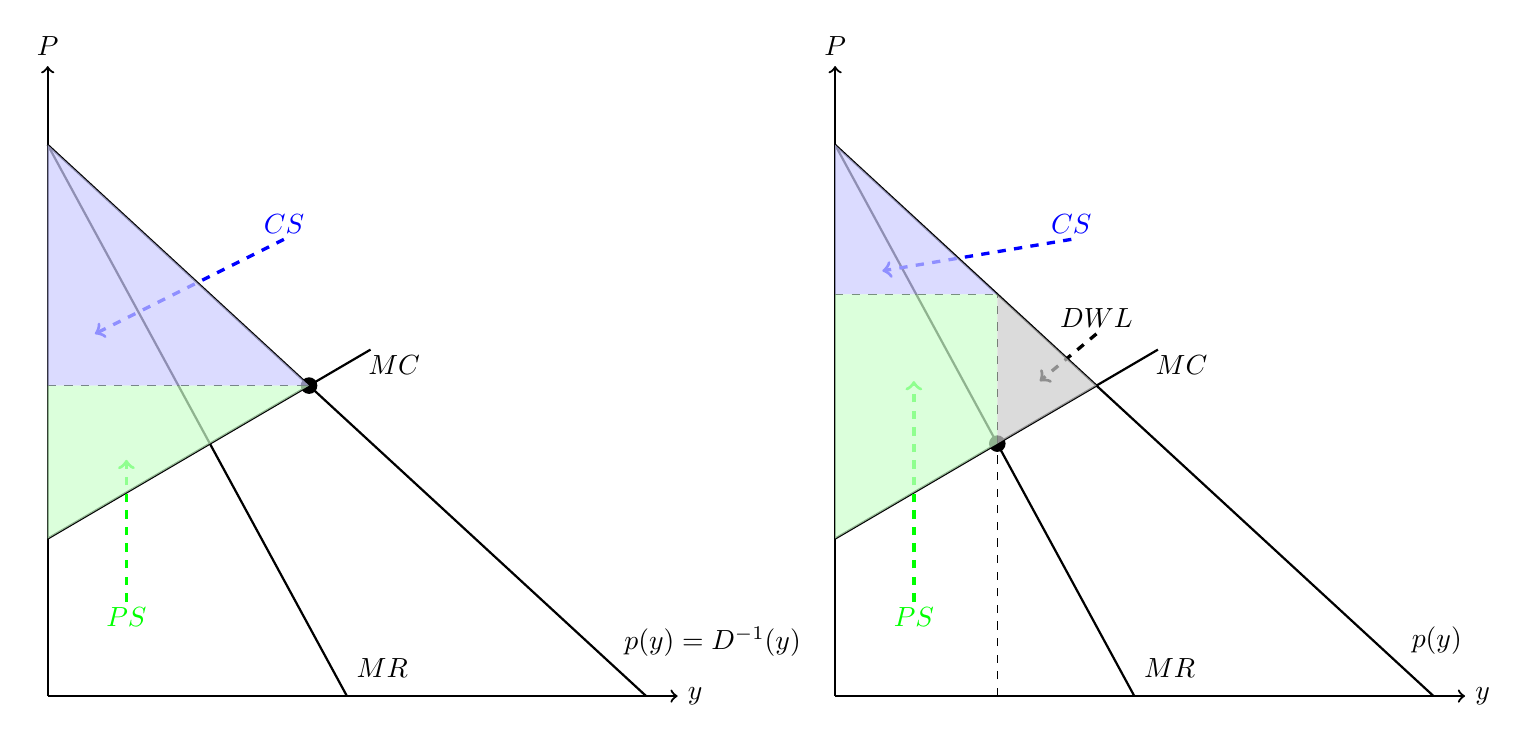
\begin{tikzpicture}[scale=2]

    \draw[thick,->] (0,0) -- (4,0) node[right] {$y$}; 
    \draw[thick,->] (0,0) -- (0,4) node[above] {$P$};

    \draw[thick, black] (0,3.5) -- (1.9,0); 
    \draw[thick, black] (0,1) -- (2.05,2.2); 
    \draw[thick, black] (0,3.5) -- (3.8,0);
    \draw[very thick, dashed, blue, ->] (1.5,2.9) -- (0.3,2.3);
    \draw[very thick, dashed, green, ->] (0.5,0.6) -- (0.5,1.5);
    \draw[dashed] (0,1.97145) -- (1.65957, 1.97145);

    \fill[teal, black] (1.65957, 1.97145) circle (1.5pt);

    \node[anchor=north west, black] at (1.9,0.3) {$MR$};
    \node[anchor=north west, black] at (3.6,0.5) {$p(y)=D^{-1}(y)$};
    \node[black] at (2.2,2.1) {$MC$};
    \node[blue] at (1.5,3) {$CS$};
    \node[green] at (0.5,0.5) {$PS$};
    \fill[fill=blue!20,opacity=0.7] 
        (0, 1.97145) -- (1.65957, 1.97145) -- (0,3.5) -- cycle;

    \fill[fill=green!20,opacity=0.7] 
        (0, 1) -- (1.65957, 1.97145) -- (0, 1.97145) -- cycle;

    \begin{scope}[shift={(5,0)}]
        \draw[thick,->] (0,0) -- (4,0) node[right] {$y$}; 
        \draw[thick,->] (0,0) -- (0,4) node[above] {$P$};

        \draw[thick, black] (0,3.5) -- (1.9,0); 
        \draw[thick, black] (0,1) -- (2.05,2.2); 
        \draw[thick, black] (0,3.5) -- (3.8,0);
        \draw[very thick, dashed, blue, ->] (1.5,2.9) -- (0.3,2.7);
        \draw[very thick, dashed, green, ->] (0.5,0.6) -- (0.5,2);
        \draw[dashed] (1.02988, 0) -- (1.02988, 2.55);
        \draw[dashed] (0,2.55) -- (1.02988, 2.55);
        \draw[very thick, dashed, ->] (1.65957, 2.3) -- (1.3, 2);

        \node[anchor=north west, black] at (1.9,0.3) {$MR$};
        \node[anchor=north west, black] at (3.6,0.5) {$p(y)$};
        \node[black] at (2.2,2.1) {$MC$};
        \node[blue] at (1.5,3) {$CS$};
        \node[green] at (0.5,0.5) {$PS$};
        \node[black] at (1.65957, 2.4) {$DWL$};
        \fill[teal, black] (1.02988, 1.60286) circle (1.5pt);
        

        \fill[fill=blue!20,opacity=0.7] 
            (0, 2.55) -- (1.02988, 2.55) -- (0,3.5) -- cycle;

        \fill[fill=green!20,opacity=0.7] 
            (0, 1) --(0, 2.55)-- (1.02988, 2.55) --(1.02988, 1.60286)-- cycle;

        \fill[fill=black!20,opacity=0.7] 
            (1.02988, 1.60286) --(1.02988, 2.55)-- (1.65957, 1.97145) -- cycle;
        
    \end{scope}
    
\end{tikzpicture}
$$

\subsection{DWL formula}
\noindent
\begin{minipage}{0.5\textwidth}
    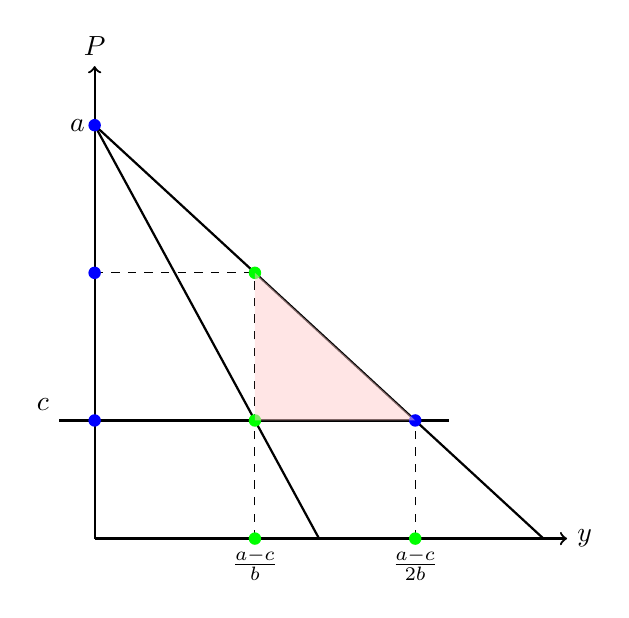
\begin{tikzpicture}[scale=1.5]
        \draw[thick,->] (0,0) -- (4,0) node[right] {$y$}; 
        \draw[thick,->] (0,0) -- (0,4) node[above] {$P$};
    
        \draw[thick, black] (0,3.5) -- (1.9,0); 
        \draw[thick, black] (-0.3,1) node[above left] {$c$} -- (3,1); 
        \draw[thick, black] (0,3.5) -- (3.8,0); %p(y)
        \draw[dashed] (1.35722, 0) -- (1.35722, 2.25);
        \draw[dashed] (0,2.25) -- (1.35722, 2.25);
        \draw[dashed] (2.71444, 0) -- (2.71444, 1);
    
        \fill[teal, green] (1.35722, 1) circle (1.5pt);
        \fill[teal, green] (1.35722, 2.25) circle (1.5pt);
        \fill[teal, blue] (2.71444, 1) circle (1.5pt);
        \fill[teal, blue] (0, 1) circle (1.5pt);
        \fill[teal, blue] (0, 3.5) circle (1.5pt) node[left, black] {$a$};
        \fill[teal, blue] (0,2.25) circle (1.5pt);
        \fill[teal, green] (1.35722, 0) circle (1.5pt) node[below, black] {$\frac{a-c}{b}$};
        \fill[teal, green] (2.71444, 0) circle (1.5pt) node[below, black] {$\frac{a-c}{2b}$};

        \fill[fill=red!20,opacity=0.5] 
            (1.35722, 1) --(1.35722, 2.25)-- (2.71444, 1) -- cycle;
    \end{tikzpicture}
\end{minipage}
\begin{minipage}{0.5\textwidth}
    For instance, we have $p(y)=a-by$ and $c'(y)=c$ then
    $$\begin{aligned}
        TR&=ay-by^2\\
        MR&=a-2by
    \end{aligned}$$

    Now, how try to find $DWL$? Optimal output will be $\hat{y}=\displaystyle\frac{a-c}{b}$, while monopoly's:
    $$y^m=\displaystyle\frac{a-c}{2b}$$
    So,
    $$DWL=\int_{y^m}^{\hat{y}}\left[(a-bt)-c\right]dt=\displaystyle\frac{(a-c)^2}{8b}$$
\end{minipage}%

\subsection{The concept of a representative consumer}
If an aggregate demand on good can be represented by solving a utility maximization problem of a sole consumer, then we say that in such economy a representative consumer exists. This is exactly the case in a quasilinear economy.

In other words there exists a function $\nu(x)$ such that by solving the problem
\begin{equation}
    \begin{cases}
        \nu(x)+\sum_{i \in I} z_i \rightarrow \max \\
        p \cdot \sum_{i \in I} x_i+\sum_{i \in I} z_i \leq \sum_{i \in I} w_i
    \end{cases}
\end{equation}
we can find the aggregate demand function $D(p) =\sum_{i\in I}x_i(p)$


\section{Regulation of a monopoly}
\begin{minipage}{0.5\textwidth}
    $$
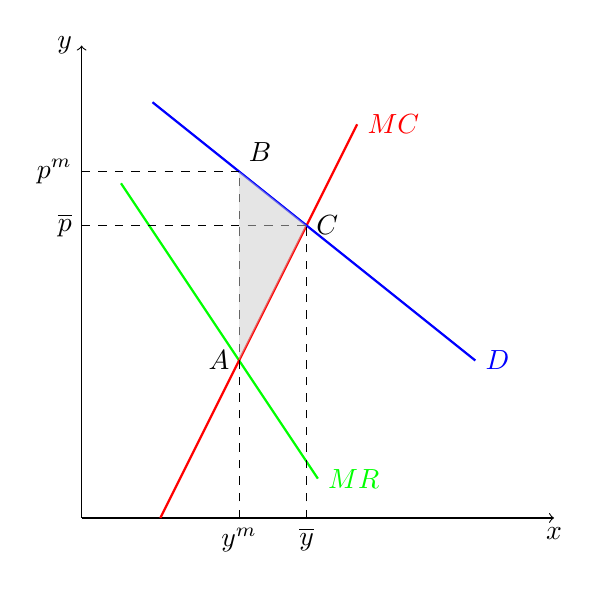
\begin{tikzpicture}
    \draw[black, ->] (0,0) -- (0,6) node[black, left] {$y$};
    \draw[black, ->] (0,0) -- (6,0) node[black, below] {$x$};
    \draw[green, thick] (0.5,4.25) -- (3, 0.5) node[green, right] {$MR$};
    \draw[red, thick] (1,0) -- (3.5,5) node[red, right] {$MC$};
    \draw[blue, thick] (0.9, 5.28) -- (5, 2) node[blue, right] {$D$};
    \draw[black, dashed] (2,0) node[black, below] {$y^m$} -- (2,4.4);
    \draw[black, dashed] (2.85714,0) node[black, below] {$\overline{y}$} -- (2.85714, 3.71429);
    \draw[black, dashed] (0,4.4) node[black, left] {$p^m$} -- (2,4.4);
    \draw[black, dashed] (0, 3.71429) node[black, left] {$\overline{p}$} -- (2.85714, 3.71429);
    \fill[fill=black!20,opacity=0.5] 
            (2,4.4) node[black!100, opacity=1, above right] {$B$} -- (2,2) node[black!100, opacity=1, left] {$A$} -- (2.85714, 3.71429)  node[black!100, opacity=1, right] {$C$} -- cycle;
    
\end{tikzpicture}
$$
\end{minipage}
\begin{minipage}{0.5\textwidth}
    $C S+P S<W_{\text {max }}$, and $D W L=$ area of the triangle ABC is greater than 0. Triangle ABC is called the Harberger's triangle. In a linear case when $p(y)=a-b y$ and $M C=c<a$
$$
D W L=\frac{(a-c)^2}{8 b}
$$

Next we'll find out that if price discrimination is allowed then $D W L$ can be reduced or even completely ceased. Monopoly regulation can be achieved via the following measures:
\begin{itemize}
    \item Price regulation
    \item Taxation of a monopoly
    \item Legal restrictions (Anti-Trust Laws)
\end{itemize}
\end{minipage}

\begin{minipage}{0.5\textwidth}
    If a concrete technology exhibits economy of scale meaning that $A C(y)$ goes down within a long range of output values compared with the demand domain (see the figure), then we call a producer a natural monopoly.\\[2mm]

    Let's imagine a firm which uses labor and capital. Then,
    $$
    \begin{aligned}
        \Pi&=TR-TC\\
        &=p(f)\cdot f - wL-rK\longrightarrow\max\limits_{L,K>0}
    \end{aligned}
    $$
    Remember, that $p(f)\cdot f$ is the function of price from the quantity multiplied by the quantity
\end{minipage}
\begin{minipage}{0.5\textwidth}
    $$
\begin{tikzpicture}
    \draw[->] (0,0) -- (7,0) node[below] {$Q$};
    \draw[->] (0,0) -- (0,6.5) node[left] {$p$};

    \draw[red, thick, domain=0.7:6] plot (\x, {3/\x}) node[right] {};

    \draw[orange, thick, domain=1:6] plot (\x, {4/(\x-0.3)}) node[right] {};

    \draw[blue, thick] (5.90909, 0) -- (1.04807, 5.34713);
    \draw[green, thick] (1.05, 3.615) -- (3.17647, 0);

    \draw[dashed] (2.45874,0) node[below] {$Q_a$} -- (2.45874,3.79539);
    \draw[dashed] (5.40445,0) node[below] {$Q_r$} -- (5.40445,0.78363);
    \draw[dashed] (0,0.78363) node[left] {$G$} -- (5.40445,0.78363);
    \draw[dashed] (0,3.79539) node[left] {$p_a$} -- (2.45874,3.79539);
    \draw[dashed] (0,0.55511) node[left] {$p_r$} -- (5.40445,0.55511);
    \draw[dashed] (0,1.85293) node[left] {$C$} -- (2.45874,1.85293);


    \fill[teal, black] (2.45874,3.79539) node[black, above right] {$A$} circle (1.5pt);
    \fill[teal, black] (2.45874,1.85293) node[black, above right] {$B$} circle (1.5pt);
    \fill[teal, black] (5.40445,0.78363) node[black, above right] {$F$} circle (1.5pt);
    \fill[teal, black] (5.40445,0.55511) node[black, below left] {$E$} circle (1.5pt);

    \node[draw, anchor=north east,fill=white] at (9,5) {
    \begin{tikzpicture}
        \draw[blue, thick] (0,0) -- (0.5,0) node[right, text=black] {\(D\)};
        \draw[green, thick] (0,-0.5) -- (0.5,-0.5) node[right, text=black] {\(MR\)};
        \draw[orange, thick] (0,-1) -- (0.5,-1) node[right, text=black] {\(AC\)};
        \draw[red, thick] (0,-1.5) -- (0.5,-1.5) node[right, text=black] {\(MC\)};
    \end{tikzpicture}
    };
\end{tikzpicture}
$$
\end{minipage}

Regulation on the basis of marginal costs is not viable here as profit will be below 0 .

Discrimination may help, or setting <<a fair return rate on the capital>>. In the latter case this measure induces a monopoly to overemploy capital.


\section{Discriminating monopoly}
If it's not forbidden by the regulating authority price discrimination is \textbf{beneficial} for monopoly itself.

\definition Price schedule is calles \textbf{linear} if for some $p>0$ the payment charged by a monopolist is $t=py$, where $y$ represents an amount sold. All other price schedules are \textit{nonlinear}

There are three types of discrimination in monopoly:
\begin{enumerate}
    \item Perfect discrimination
    \item Nonlinear pricing schedule
    \item Segmentation of the market
\end{enumerate}

Moreover, \textbf{arbitrage} is forbidden, which means that consumers can't sell good to each other


\subsection{First kind of discrimination. Perfect model}
According to Arthur Pigou at discrimination of this type a monopoly may charge different prices to different consumers and pricing is nonlinear\dots

It is worth mentioning that the monopoly has to have \textit{perfect knowledge} about the market and utility functions of consumers.


\subsubsection{The model of discrimination}
Let $i \in I$ and $U_i\left(x_i, z_i\right)=\nu_i\left(x_i\right)+z_i$, where $\nu_i^{\prime}>0, \nu_i^{\prime \prime}<0$ and $\nu_i(0)=0$. Money endowments are $w_i>0$.

Remember, that $I$ is a set of indices.

Let monopoly offers $x_i$ amount to the $i$-th consumer and charges $t_i$. 

Let $c(y)$ be the costs function with the properties $c^{\prime}(y)>0$, $c^{\prime \prime}(y)>0$.

We call \textit{participation constraint} inequality
$$
\begin{aligned}
    \nu_i\left(x_i\right)-t_i &\geqslant \nu_i(0)\\
    &\geqslant 0\ \forall i \in I
\end{aligned}
$$

If this inequality is strict the bargain will satisfy the consumer, but even if $\nu_i\left(x_i\right)=t_i$, still the deal can be struck.

\subsubsection{Maximization problem}
From the previous part we set maximization problem:
\begin{equation*}
    \begin{cases}
        \Pi=\sum_{i\in I}t_i-c\left(\sum_{i\in I} x_i\right)\longrightarrow\max_{t_i,x_i\geqslant0}\\
        \nu_i(x_i)\geqslant t_i\ \forall i
    \end{cases}
\end{equation*}

The monopoly wants to set maximum price for each consumer that is why:
\begin{equation*}
    \nu_i(x_i)=t_i\ \forall i
\end{equation*}
So, we transform our problem to
\begin{equation*}
    \Pi=\sum_{i\in I}\mu_i(x_i)-c\left(\sum_{i\in I} x_i\right)\longrightarrow\max_{x_i\geqslant0}
\end{equation*}

$$
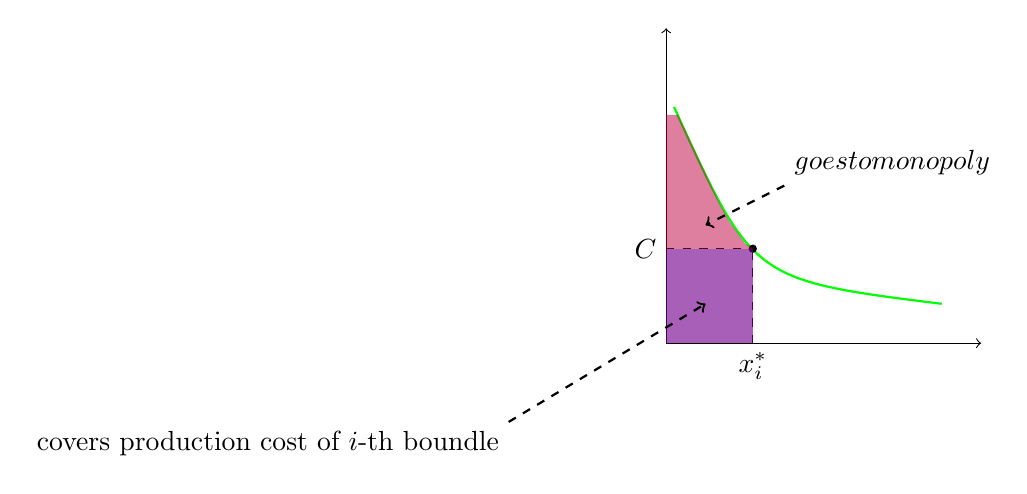
\begin{tikzpicture}
    
    \draw[black, ->] (0,0) -- (0,4);
    \draw[black, ->] (0,0) -- (4,0);
    \draw[thick, green] (0.1,3) .. controls (1.1,0.8) .. (3.5,0.5);
    \draw[black, dashed] (1.1,0) node[black, below] {$x_i^*$} -- (1.1,1.2);
    \draw[black, dashed] (0,1.2) node[black, left] {$C$} -- (1.1,1.2);
    \fill[teal, black] (1.1,1.2) circle (1.5pt);
    \fill[purple, opacity=0.5] (0,0) -- (1.1,0) -- (1.1,1.2) -- (1,1.27) -- (0.95,1.34) -- (0.9, 1.41) --  (0.85, 1.48) --  (0.8, 1.55) --  (0.75, 1.65) --  (0.7, 1.73) -- (0.15,2.9) -- (0,2.9) -- (0,0) -- cycle;
    
    \fill[blue, opacity=0.25] (0,0) -- (1.1,0) -- (1.1,1.2) -- (0,1.2) -- (0,0) -- cycle;
    \draw[dashed, black, thick, ->] (1.5, 2) node[black, above right] {$\text{goes to monopoly}$} -- (0.5,1.5);
    \draw[dashed, black, thick, ->] (-2, -1) -- (0.5,0.5);
    \node[black, below left] at (-2, -1) {covers production cost of $i$-th boundle};
\end{tikzpicture}
$$

\subsubsection{Take-it-or-leave-it}
It's the scheme of payment when the monopoly suggests consumers to buy $x$ of the good by the price $t$. If you don't accept it, you'll leave the market. In this case the emonopoly will not get and will not lose anything. The scheme can be displayed by next function:
\begin{equation*}
    t(x)=\begin{cases}
        t^*,&x\leqslant x^*\\
        +\infty, & x>x^*
    \end{cases}
\end{equation*}


\subsection{Second kind of discrimination. Nonlinear pricing}
Here we will be looking over two subtypes of the second kind od discrimination: package deals and two-part tariff. Imagine that we have two consumers: Mr.High and Mr.Low. By the way, 
\begin{equation*}
    \forall x:\ v^\prime_l(x) < v^\prime_h
\end{equation*}
and if $v^\prime(0)=0$ $(i=l,h)$, then
\begin{equation*}
    v_l(x) < v_h(x)\ \forall x>0
\end{equation*}

\subsubsection{Package deals}
This type is similiar to the scheme \textit{take-it-or-leave-it}. Let $I=\{1\}$. Then $U(x,z)=\nu(x)+z$. In taht case a consumer will solve the problem
\begin{equation*}
    \begin{cases}
        \nu(x)+z\longrightarrow\max\limits_{x,z\geqslant0}\\
        t(x)+z\leqslant w\\
        t,z,x\geqslant 0
    \end{cases}
\end{equation*}

Monopolist gets (the deal is struck) then maximized
\begin{equation*}
    \Pi(x)=\nu(x)-c(x)
\end{equation*}

\subsubsection{Two-part tariff}
The main idea of this scheme is that a consumer pays twice. The first price $A>0$ for probability to buy (we can call it <<admission fee>>) and the second one is proportional to the quantity of goods. More formally:
\begin{equation*}
    t(x)=\begin{cases}
        A+px&x>0\\
        0&x=0
    \end{cases}
\end{equation*}

The entry payment and per-unit price $p$, and $x^*$ — the solution of the consumer problem:
\begin{equation*}
    \begin{cases}
        \nu(x)+z\longrightarrow\max\limits_{x,z}\\
        A+px+z\leqslant w\\
        A,x,z\geqslant 0
    \end{cases}
\end{equation*}
Then $z=w-A-px$ and $\nu(x)+w-A-p x \longrightarrow \max\limits_{x>0} \Longrightarrow \nu^{\prime}\left(x^*\right)=p$.

Monopoly problem:
$$
\Pi(x)=A+p \cdot x-c \cdot x \longrightarrow \max\limits_{x\geqslant 0}
$$

Then $p^*=c$ (like in perfect competition) and since 
$$\nu\left(x^*\right)-A-c \cdot x^*+w=w$$
then 
$$A=C S=\int_0^{x^*}\left[\nu^{\prime}(z)-c\right]\d{x}$$

Once again the consumer surplus is drawn from a consumer to monopoly. This kind of discrimination is not achievable!

% $$TWO\ ILLUSTRATIONS\ FROM\ SUMMARY$$

\subsubsection{Two consumers}
Also, we can represent this kind of discrimination to 2 consumers — High and Low, and offer them 2 packages: $(x_l,t_l), (x_h,t_h)$: each package is personalized per each consumer

$$
\begin{aligned}
    U_h(x, z)=\nu_h(x)&+z \\
    U_l(x, z)=\nu_l(x)&+z
\end{aligned}
$$

Applying the first discrimination pricing for them is not possible since the high agent pretends to be the low agent and that claim enables her to keep part of her $CS$.

$$
\begin{tikzpicture}
    \draw[->] (0,0) -- (7,0) node[below] {$x$};
    \draw[->] (0,0) -- (0,5) node[left] {$p$};

    \draw[blue, thick, domain=0.7:6] plot (\x, {3/\x}) node[right] {};

    \draw[green, thick, domain=1.3:6] plot (\x, {4/(\x-0.3)}) node[right] {};

    \draw[red, thick] (0,1.8) -- (7,1.8);

    \draw[dashed] (1.66667,0) node[below] {$x_l^*$} -- (1.66667, 2.92682);
    \draw[dashed] (2.52222,0) node[below] {$x_h^*$} -- (2.52222, 1.8);

    \node at (0.7,2.5) {B};
    \node at (1,1) {A};
    \node at (1.4,2.7) {C};
    \node at (2,0.56) {D};
    \node at (2,2.1) {F};
    \node at (2.3,1.5) {E};

    \node[draw, anchor=north east,fill=white] at (9,5) {
    \begin{tikzpicture}
        \draw[blue, thick] (0,0) -- (0.5,0) node[right, text=black] {\(v^{\prime}_l(x)\)};
        \draw[green, thick] (0,-0.5) -- (0.5,-0.5) node[right, text=black] {\(v^{\prime}_h(x)\)};
        \draw[red, thick] (0,-1) -- (0.5,-1) node[right, text=black] {\(MC\)};
    \end{tikzpicture}
    };
\end{tikzpicture}
$$


\subsection{Third kind of discrimination. Segmentation of the market}
Suppose a market is split in $m$ submarkets and monopoly faces $D_i(p)=x_i i \in\{1, \ldots, m\}$ demand on each of them.

Then by setting $p_i$ on the $i$-th segment of the market, the monopoly price discriminates between them.

A monopoly can differentiate the market on some groups. Then a monopoly should follow the rule <<to each group — each price>>


\proposition Let $p_i$ and $p_j$ be prices charged by monopoly on respectively $i$-th and $j$-th segments. Then
$$
\frac{p_i}{p_j}=\frac{1-\frac{1}{\left|\varepsilon_j\left(p_j\right)\right|}}{1-\frac{1}{\left|\varepsilon_i\left(p_i\right)\right|}}
$$
where $\varepsilon_i$ and $\varepsilon_j$ are the respective price elasticities.

As we have seen discriminations of the first and second kinds either eliminate $DWL$ completely or reduce it.

But in case of third kind discrimination the situation is different. It follows from the following.


\section{Discriminating—2}
\corollary If the total output \textit{does not} increase when a monopoly moves from nondiscrimination to discrimination, the \textbf{total social welfare can't go up.}

When we deal with the linear demands $D_i(p)=a_i-b_i p$ and $M C=c<\min a_i$ for $i \in \overline{1, m}$ the output of a non-discriminating and discriminating monopoly is the same, given that $D_i(\bar{p})>0$ for $i \in \overline{1, m}$.

Now we can construct two segments (non-discriminating and discriminating) when $D W L^{n d}<D W L^d$. Let's prove for linear case:

\begin{itemize}
    \item \textit{Non-discriminating.} 
    \begin{equation*}
        \begin{aligned}
            p=a-by &\text{ and }\Pi=(a-by)y-cy\longrightarrow\max\limits_{y\geqslant0}\\
            &a-c-2by\geqslant0
        \end{aligned}
    \end{equation*}
    \item \textit{Discriminating.}
    \begin{equation*}
        \begin{aligned}
            p_i=a_i-b_iy_i\Longrightarrow y_i\frac{a_i-p}{b_i}
        \end{aligned}
    \end{equation*}
    Summing up by all submarkets we'll get a demand function
    $$y(p)=\sum_{i=1}^k y_i(p)=\sum_{i=1}^k \frac{a_i}{b_i}-\left(\sum_{i \in I} \frac{1}{b_i}\right) p$$
    Inverse demand function
    $$p(y)=\frac{\sum_{i \in I} a_i / b_i}{\sum_{i \in I} 1 / b_i}-\frac{1}{\sum_{i \in I} 1 / b_i} y$$
    then
    $$y^*=\frac{1}{2}\left(\sum_{i \in I} \frac{a_i}{b_i}-c \sum_{i \in I} \frac{1}{b_i}\right)$$

    When discriminating by submarkets, the monopolist sells in the i-th submarket:
    $$\tilde{y}_i=\frac{a_i-c}{2 b_i}$$
    Summing up by all submarkets we'll get
    $$\sum_{i=1}^k \tilde{y}_i=\sum_{i=1}^k \frac{a_i-c}{2 b_i}=\frac{1}{2}\left(\sum_{i \in I} \frac{a_i}{b_i}-c \sum_{i \in I} \frac{1}{b_i}\right)$$
\end{itemize}



\begin{minipage}{0.5\textwidth}
    \proposition Let $\bar{p}$ be a uniform (non-discriminating) price and $\tilde{p_i}$ a price charged on $i$-th segment.

Compare two values of the welfare indicator:
$$
\begin{gathered}
W(\bar{p})=\sum_{i=1}^m \nu_i\left(D_i(\bar{p})\right)-c \sum_{i=1}^m D_i(\bar{p}) \\
\text { and } \\
W\left(\tilde{p_1}, \ldots, \tilde{p_m}\right)=\sum_{i=1}^m \nu_i\left(D_i\left(\tilde{p_i}\right)\right)-c \sum_{i=1}^m D_i\left(\tilde{p_i}\right)
\end{gathered}
$$
where $\nu_i(x)$ are components of the utilities, then
$$
W\left(\tilde{p_1}, \ldots, \tilde{p_m}\right) \leqslant(\bar{p}-c) \sum_{i=1}^m \Delta y_i,\text{ where }\Delta y_i=D_i\left(\tilde{p}_i\right)-D_i(\bar{p})
$$
\end{minipage}
\begin{minipage}{0.5\textwidth}
    $$
\begin{tikzpicture}
    \draw[->] (0,0) -- (5,0) node[below] {$x$};
    \draw[->] (0,0) -- (0,5) node[left] {$p$};

    \draw[blue, thick, domain=0:4] plot (\x, {-(0.5*\x-1.7320508)^2+3}) node[right] {};

    \draw[green, thick, domain=0:3.5] plot (\x, {0.732*\x+0.996}) node[right] {};

    \draw[black, dashed] (2,0) node[below] {$x_0$} -- (2,2.46);
    \draw[black, dashed] (3,0) node[below] {$x$}  -- (3, 2.94615);
    \fill[teal, black] (2, 2.46) circle (1.5pt);
    \fill[teal, black] (3, 2.94615) circle (1.5pt);
    \draw[black] (2,2.46) -- (3,2.46);
    \draw[black] (3,2.46) -- (3, 2.94615);
\end{tikzpicture}
$$
$$f(x)-f(x_0)\leqslant f'(x_0)f(x-x_0)$$
\end{minipage}

\subsection{Weeping willow}
<<Weeping willow>> is the only restaurant to sell alcohol. 

The demand: $x(p,t)=1-p+t$, where $t$ — time since the restauranthas been opened (per day), i.e. $0\leqslant t\leqslant1$. Then $MC=\frac{1}{2}$

Let's solve the profit maximization problem:
\begin{equation*}
    \begin{aligned}
        \Pi(p)&=\left(p-\frac{1}{2}\right)\int_0^{\frac{1}{2}}\d{t}\\
        \Pi^{\prime}&=\left[(p-\frac{1}{2})(\frac{3}{2}-p)\right]\\
        &=\frac{3}{2}-p-\left(p-\frac{1}{2}\right)\\
        &=0
    \end{aligned}
\end{equation*}
As again, the steps are:
\begin{enumerate}
    \item Profit
    \item $\Pi',\ p^*$ if $\Pi=0$
\end{enumerate}

\section{Location models of monopolistic competition}
Consumers are uniformly distributed along linear city (a beach). There are two icecream stands. Stand $A$ is located $a$ meters from the left and $B$ stand is at $b$ meters from the right. The production of an icecream is costless by after purchase the carrying it back costs $c$ dollars per unit of distance (it melts).

We need to find the prices charged by the stands.

Then $P_A+c x=P_B+c y$. And if we add all the linear segments we get $a+x+y+b=L$.
We get a system of 2 equations. After solving we get
$$
\left\{\begin{array}{l}
x=\frac{1}{2}\left(L-a-b+\frac{P_B-P_A}{c}\right) \\
y=\frac{1}{2}\left(L-a-b+\frac{P_A-P_B}{c}\right)
\end{array}\right.
$$

Then we need to find the profits
$$
\begin{aligned}
& \pi_A=\frac{1}{2}(L+a-b) P_A+\frac{P_A P_B-P_A^2}{2 c} \\
& \pi_B=\frac{1}{2}(L-a+b) P_B+\frac{P_A P_B-P_B^2}{2 c}
\end{aligned}
$$

Maximizing both profits with respect to the prices will gives the prices
$$
\begin{aligned}
P_A & =c\left(L+\frac{a-b}{3}\right) \\
P_B & =c\left(L-\frac{a-b}{3}\right)
\end{aligned}
$$

\section{Game theory}
\definition Simultaneous game — is a game in which a single decision is made by each player, and each player has no knowledge of other player decisions before the game.

Said this we do not exclude the expectations of decisions that may or may not be realized.

To describe such a game we need to specify:
\begin{itemize}
    \item the set of players indexed by $i \in I$;
    \item a strategy set $S_i$ for each player;
    \item payoffs for each player for any combination of strategies used by all players.
\end{itemize}

\subsection{Prisoners' dilemma}
There are two players $P_1$ and $P_2$ who choose actions $C$ (cooperate) or $D$ (defect).

Their payoffs are in the following table:
$$\begin{array}{c|c|c} 
    & C & D \\ \hline
    C & 3,3 & 0,5 \\ \hline
    D & 5,0 & 1,1 \\
  \end{array}
$$

Clearly $(D, D)$ that provide less payoffs compared with $(C, C)$. We say that $(D, D)$ is \textbf{Pareto inefficient equilibrium} (Pareto optimality is used here in the same sense like in exchange theory).

When a game is described in a tabular form, we say that this is \textbf{normal form} of a game.

\subsection{Nash equilibrium in pure strategies}
\definition NE for 2 players is a pair of strategies $\left(\sigma_1^*, \sigma_2^*\right)$ such that
$$
\begin{gathered}
\pi_1\left(\sigma_1^*, \sigma_2^*\right) \geqslant \pi_1\left(\sigma_1, \sigma_2^*\right) \\
\forall \sigma_1 \in S_1 \\
\pi_2\left(\sigma_1^*, \sigma_2^*\right) \geqslant \pi_2\left(\sigma_1^*, \sigma_2\right) \\
\forall \sigma_2 \in S_2
\end{gathered}
$$

Here $\pi_1, \pi_2$ are payoffs of the players and $S_1, S_2$ are respective sets of strategies.


\subsection{Dominance solvable games}
A strategy for player $1 \sigma_1$ is strictly dominated by $\sigma_1^{\prime}$ if
$$
\begin{gathered}
\pi\left(\sigma_1^{\prime}, \sigma_2\right)>\pi\left(\sigma_1, \sigma_2\right) \\
\forall \sigma_2 \in S_2
\end{gathered}
$$

When inequality is nonstrict we call such a dominance weak.

Strictly dominated strategies are not played.

\subsection{Theory of the best response}
\definition Let the set $S$ of strategies of a player consists of $S=\left\{s_a, s_b, s_c, \ldots\right\}$.

Then a mixed strategy can be represented as a vector of probabilities $\sigma=\left(p\left(s_a\right), p\left(s_b\right), p\left(s_c\right), \ldots\right)$.

We consider
$$
\pi_i\left(\sigma_1, \sigma_2\right)=\sum_{s_1 \in S_1} \sum_{s_2 \in S_2} p\left(s_1\right) q\left(s_2\right) \pi_i\left(s_1, s_2\right)
$$

\definition A pair of strategies $\left(\sigma_1^*, \sigma_2^*\right)$ is a $NE$ (=is the best response) if
$$\begin{aligned}
    \begin{gathered}
    \sigma_1^* \in \arg \max _{\sigma_1} \pi_1\left(\sigma_1, \sigma_2^*\right) \\
    \text { and } \\
    \sigma_2^* \in \arg \max _{\sigma_2} \pi_2\left(\sigma_1^*, \sigma_2\right)
    \end{gathered}
    \end{aligned}
$$


\section{Oligopoly}
\definition An oligopoly — is a market structure in which a small number of firms dominate the industry. 

These firms have significant control over pricing and supply, and their decisions can greatly influence the market. 

In an oligopoly, companies may compete or collaborate, and the actions of one firm often impact the others. This market structure typically results in limited competition and can lead to higher prices or less innovation compared to more competitive markets.

\subsection{Cournot model}
I don't fucking care what is going on next. I'm done. Sorry, I'll add it later






\end{document}